\level{2}{Processo di configurazione}
	\level{3}{Norme}
			\level{4}{Controllo di versione}
				Il controllo sul versionamento dei documenti e, nelle successive fasi del progetto, dei codici sorgente avviene attraverso lo strumento fornito dalla piattaforma GitHub.\\
				Ogni volta che viene eseguita una modifica sostanziale deve essere assegnato un nuovo numero di versione.\\
				Per quanto riguarda le norme riguardanti il versionamento della documentazione si rimanda alla sezione \hyperref[sec:versioni]{Versionamento dei documenti} del presente documento.
				\level{4}{Struttura di una richiesta di modifica}
					Ogni richiesta di modifica è costituita dai seguenti campi:
					\begin{enumerate}
						\item autore: contiene nome e cognome di colui che richiede la modifica;
						\item documento: contiene il nome del documento di cui si richiede la modifica;
						\item motivo: contiene la spiegazione chiara e concisa delle motivazioni per cui si sta richiedendo una modifica;
						\item urgenza: può assumere uno dei seguenti valori:
							\begin{enumerate}
								\item alta: si tratta di una modifica importante, con forti conseguenze nell'organizzazione e nello svolgimento delle attività future del progetto;
								\item media: si tratta di una modifica importante, ma che non comporta grandi modifiche alle attività del progetto;
								\item bassa: si tratta di una modifica di importanza secondaria, che può essere rimandata ad un secondo momento senza che ciò influisca in alcun modo sullo svolgimento delle attività.
							\end{enumerate}
					In seguito alla decisione del \insrole{Responsabile} di approvare o meno la richiesta, va aggiunto il campo:
						\item Decisione del \insrole{Responsabile di Progetto}: contiene uno dei seguenti valori:
							\begin{enumerate}
								\item approvata;
								\item respinta.
							\end{enumerate}
					\end{enumerate}
		
				\level{4}{Struttura del repository}
					I file all’interno del repository sono organizzati secondo la seguente struttura:
					\begin{itemize}
						\item /Documents
						\begin{itemize}
							\item Commons
							\item NormeDiProgetto
							\item StudioDiFattibilità
							\item AnalisiDeiRequisiti
							\item PianoDiProgetto
							\item PianoDiQualifica
							\item SpecificaTecnica
							\item Verbali
							\item Glossario
						\end{itemize}
						\item /Source
					\end{itemize}
					La struttura di /Source viene definita prima della progettazione architetturale.

				\level{4}{Nomi dei file}
					I nomi dei file all’interno del repository sono soggetti alle seguenti norme:
					\begin{itemize}
						\item devono contenere solamente lettere, numeri, il carattere underscore U+005F, il segno meno U+2212 e il punto U+002E;
						\item devono avere una lunghezza minima di 3 caratteri;
						\item devono contenere le informazioni sufficienti per distinguere il file in modo non ambiguo;
						\item le informazioni devono essere riportate dal generale al particolare;
						\item le date devono essere specificate nel formato YYYYMMDD.
					\end{itemize}
					Si consiglia inoltre:
					\begin{itemize}
						\item di utilizzare il meno possibile i caratteri underscore e segno meno, utilizzando al loro posto la notazione camel case;
						\item di utilizzare nomi con una lunghezza compresa tra i 5 e i 25 caratteri;
						\item di specificare sempre l’estensione quando possibile.
					\end{itemize}
				\level{4}{Commit}
					L'esecuzione di un comando di commit implica il rispetto delle seguenti norme:
					\begin{itemize}
						\item quando si effettua un commit è necessario specificare nel messaggio una descrizione sintetica e non ambigua delle modifiche apportate;
						\item le modifiche apportate con un commit devono essere complete e testate con successo;
						\item le modifiche apportate con un commit devono essere logicamente correlate tra di loro.
					\end{itemize}
				\level{4}{Codifica dei file}
					Tutti i file contenenti codice o documentazione dovranno utilizzare la codifica UTF-8 senza BOM.\\
					Il terminatore di linea è il carattere Line Feed, rappresentato dal carattere Unicode U+000A.
		
		\level{3}{Procedure}
			\level{4}{Richiesta di modifica}
				Ogni richiesta di modifica va inoltrata in modo formale al \insrole{Responsabile di Progetto}, affinché venga sottoposta ad un rigoroso processo di analisi. Dopodiché il \insrole{Responsabile di Progetto} decide se approvarla o meno. Nel primo caso assegna la realizzazione della modifica ad un membro del gruppo. 
				La procedura viene formalizzata nel seguente diagramma delle attività:
				\begin{figure}[H]
					\centering
					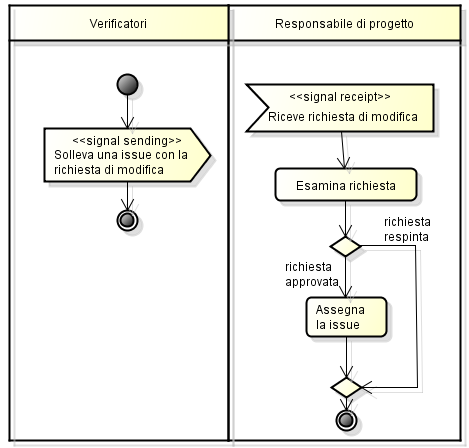
\includegraphics[width=0.6\textwidth]{NormeDiProgetto/Pics/RichiestaDiModifica}
					\caption{Procedura di richiesta di modifica}
				\end{figure}
			
			\level{4}{Aggiornamento del repository}
					Per aggiornare il repository è nesessario seguire correttamente la seguente procedura:
					\begin{enumerate}
						\item si esegue il comando git pull per aggiornare il repository locale alla commit più recente;
						\item se sono avvenuti conflitti si passa al punto (3), altimenti si prosegue col punto (4);
						\item con il comando git stash è possibile salvare le modifiche incomplete in uno stack separato per poterle riutilizzare in seguito; dopo aver accantonato i file è necessario aggiornare il repository col comando git pull, in questo modo si ha una directory di lavoro "pulita" e si possono inserire le modifiche prima accantonate;
						\item si scelgono i file di cui fare il commit usando il comando git add;
						\item si esegue il comando git commit;
						\item si esegue git push per inviare le modifiche effettuate al repository remoto;
						\item se il comando push fallisce si prosegue col punto (8), altrimenti si passa al punto (9);
						\item si riaggiorna il repository locale tramite git pull, il quale creerà un merge commit, dopo di che si riesegue il comando push (si veda il punto (7));
						\item il repository remoto è stato aggiornato.
					\end{enumerate}
					Si riporta la formalizzazione della procedura con un diagramma delle attività:
					\begin{figure}[H]
						\centering
						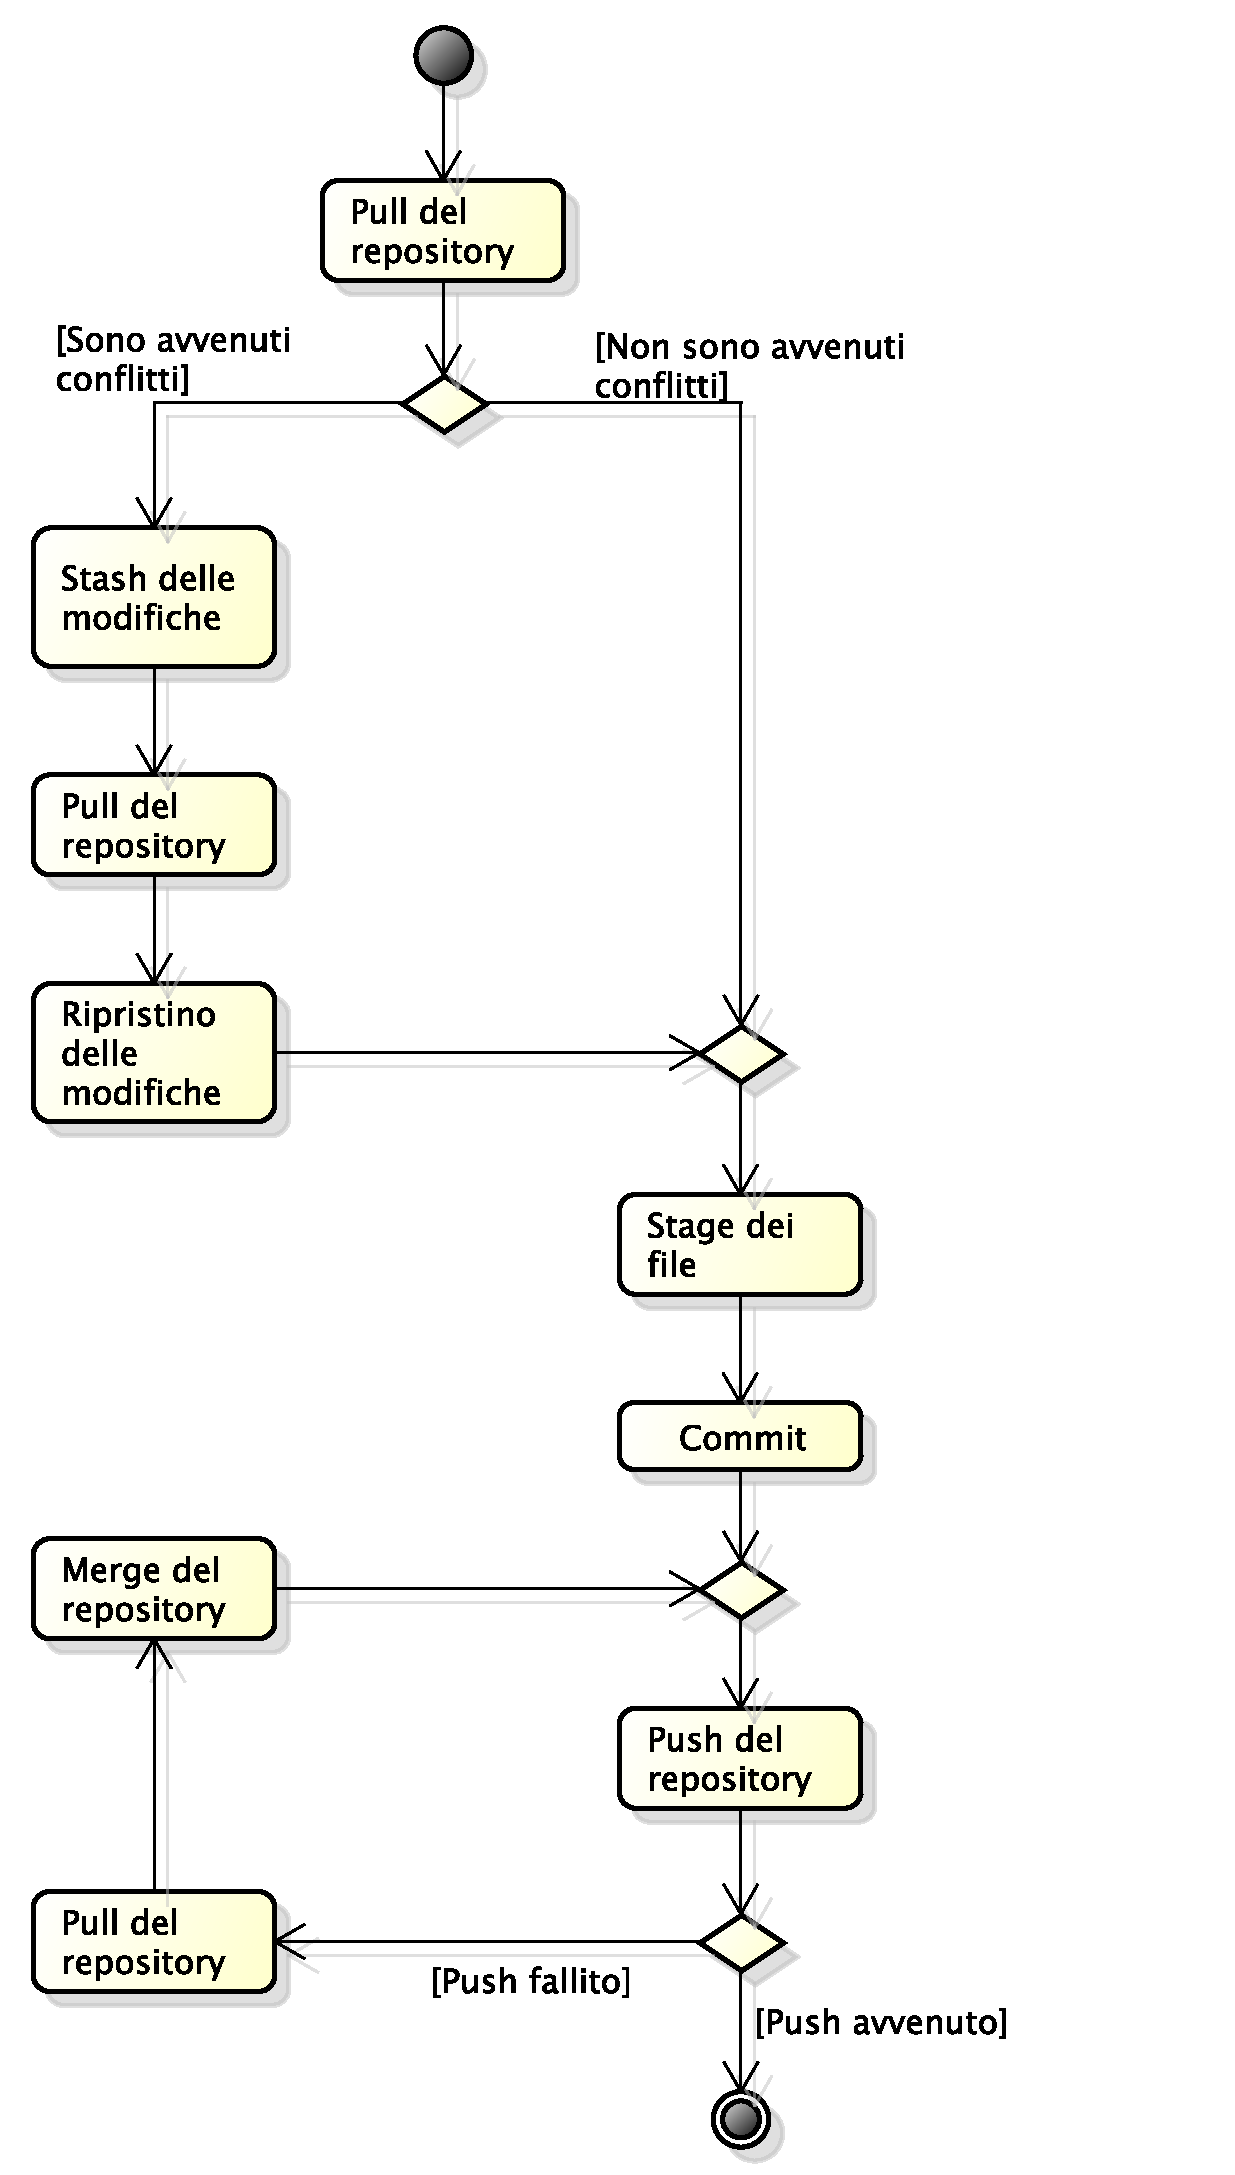
\includegraphics[width=0.6\textwidth]{NormeDiProgetto/Pics/Commit}
						\caption{Procedura di aggiornamento del repository}
					\end{figure}
	\level{3}{Strumenti}
			Per agevolare lo svolgimento del progetto da parte di tutti i membri del team di sviluppo è stata predisposta una macchina virtuale contenente tutti gli strumenti software necessari, individuati fino al momento della stesura dell'ultima versione attuale del presente documento.
			Per la gestione del repository si è scelto di utilizzare il sistema di versionamento distribuito Git, mentre per la condivisione e il versionamento dei \textit{configuration item} è stato creato un repository privato su GitHub.
			L'utilizzo dei sistemi Git e GitHub è descritto nell'appendice \nameref{app:strumenti}.
